\chapter{IMPLEMENTATION AND DEPLOYMENT}
\label{ch:implementation}

\section{IMPLEMENTATION OVERVIEW}

The previous chapter defined the design: one schema, one scoring function, two estimators that fit nothing across cells, and explicit refusals. This chapter describes how that design was realised. The implementation has three parts:

\begin{itemize}
    \item \textbf{Part A -- Telemetry and estimation software:} the packages that acquire, validate, segment and score telemetry (Sections~\ref{sec:impl-env} to~\ref{sec:impl-gates}).
    \item \textbf{Part B -- Hardware bench rig:} the instrumentation design, firmware and physical bring-up that supply real telemetry to the software (Section~\ref{sec:impl-hw}).
    \item \textbf{Part C -- Service tier and deployment:} the REST API, the gateway, the dashboard, testing, continuous integration and containers (Sections~\ref{sec:impl-api} to~\ref{sec:impl-deploy}).
\end{itemize}

\section{DEVELOPMENT ENVIRONMENT AND TOOLS}
\label{sec:impl-env}

The system is written in Python, Node (JavaScript), React and C++ (Arduino firmware), with about 23,000 lines of Python in the core package and 44 test modules. The components that matter for reproducibility are listed in Table~\ref{tab:software}.

\begin{table}[htbp]
	\caption{Software Components Used}
	\centering
	\small
	\renewcommand{\arraystretch}{1.15}
	\setlength{\tabcolsep}{4pt}
	\begin{tabular}{|L{0.27\linewidth}|L{0.57\linewidth}|}
		\hline
		\textbf{Software} & \textbf{Role} \\
		\hline
		Python ($\ge$3.10) & Core language; CI tests 3.10 (the declared floor) and 3.12 \\
		\hline
		pandas, NumPy, scikit-learn & Telemetry frames, numerical work, benchmark estimators and bootstrap analysis \\
		\hline
		XGBoost, PyTorch (optional) & Benchmark methods (gradient boosting, LSTM) \\
		\hline
		FastAPI, uvicorn & Scoring, telemetry ingest and fleet store as a REST service \\
		\hline
		cantools, python-can (optional) & DBC decoding and CAN capture; CI also runs the suite with them uninstalled \\
		\hline
		pyserial (optional) & Reading the physical rig's serial port \\
		\hline
		Express (Node) & Gateway between the client and the Python service \\
		\hline
		React, Vite & Dashboard client \\
		\hline
		Arduino C++ / \texttt{arduino-cli} & Rig firmware, compiled for ESP32, ESP8266 and AVR \\
		\hline
		pytest, ruff, mypy & Tests, linting and type checking \\
		\hline
		Docker, Docker Compose & Multi-stage image and three-service stack \\
		\hline
		GitHub Actions & Eight CI jobs, including a reproduction of the headline study \\
		\hline
	\end{tabular}
	\label{tab:software}
\end{table}

\section{CODE ORGANISATION}
\label{sec:impl-org}

The core package \texttt{src/bms} is divided into packages with one responsibility each (Table~\ref{tab:packages}).

\begin{table}[htbp]
	\caption{Organisation of the Core Package}
	\centering
	\small
	\renewcommand{\arraystretch}{1.15}
	\setlength{\tabcolsep}{4pt}
	\begin{tabular}{|L{0.22\linewidth}|L{0.64\linewidth}|}
		\hline
		\textbf{Package} & \textbf{Responsibility} \\
		\hline
		\texttt{telemetry} & CAN capture and replay, serial ingestion and protocol, cycle segmentation, and the shared scoring function \\
		\hline
		\texttt{io} & Dataset loaders (NASA, CALCE, Oxford) and DBC examples; the unified schema is in \texttt{preprocessing} \\
		\hline
		\texttt{features}, \texttt{preprocessing} & Behaviour features and data conditioning \\
		\hline
		\texttt{risk}, \texttt{health} & Rule-based risk and health index (heuristic layer); measured field SOH, voltage-window, evidence and error-band estimators \\
		\hline
		\texttt{rul} & Fade-extrapolation remaining useful life, and the earlier heuristic estimate \\
		\hline
		\texttt{guardian}, \texttt{digital\_twin} & Human-readable diagnosis and the state-machine twin \\
		\hline
		\texttt{explain} & Exact Shapley attribution over the rule scores \\
		\hline
		\texttt{uncertainty} & Distribution-free uncertainty (conformal prediction) and coverage under shift \\
		\hline
		\texttt{benchmarks} & Published methods run through the project's own validation gate \\
		\hline
		\texttt{adaptive} & Governed model promotion across datasets and protocols \\
		\hline
		\texttt{detect}, \texttt{physics} & Unsupervised usage segmentation; physics-grounded degradation models \\
		\hline
		\texttt{simulation} & Synthetic telemetry for tests and the no-hardware demo \\
		\hline
		\texttt{api}, \texttt{dashboard} & FastAPI service and the static HTML dashboard \\
		\hline
	\end{tabular}
	\label{tab:packages}
\end{table}

Outside the package, the repository holds the following.
\begin{itemize}
	\item \texttt{mern/}: the Express gateway and React client.
	\item \texttt{firmware/beacon\_rig/}: the Arduino sketch.
	\item \texttt{scripts/}: the study and demo scripts.
	\item \texttt{tests/}: the test modules.
	\item \texttt{docs/adr/}: fourteen architecture decision records, including those that record reversed decisions.
\end{itemize}

\section{TELEMETRY ACQUISITION AND THE UNIFIED FRAME}
\label{sec:impl-transports}

The three transports converge on one unified telemetry frame with the columns \texttt{cell\_id}, \texttt{test\_time\_s}, \texttt{voltage\_v}, \texttt{current\_a}, \texttt{temperature\_c} and \texttt{soc}.

\begin{itemize}
    \item \textbf{CAN bus.} Frames are decoded against a DBC definition, and a coverage gate refuses a capture whose required signals are missing.
    \item \textbf{USB serial.} A line source feeds a parser that classifies each line, verifies its checksum and validates every field against a declared range (Section~\ref{sec:impl-protocol}).
    \item \textbf{Research datasets.} Loaders read the NASA MATLAB files and the CALCE and Oxford records into the same frame.
\end{itemize}

\subsection{Interface Between Acquisition and Scoring}

A serial source is a protocol with one method, \texttt{lines()}. A physical port, a recorded text file, a list in a test and the deterministic emulator are interchangeable, so the demo path and the hardware path differ in one constructor call. The emulator deliberately generates \emph{wire-format text} and not record objects. Emitting objects would have been less code but would have proved nothing, because the parser, the checksum, the schema validation and the coverage gate would all be bypassed in exactly the path the tests exercise. The emulator even prints an ESP32 boot banner, so the sentinel filter runs on every test. Recording composes at the same seam: one decorator makes a live port, a replay or the emulator recordable, and the file on disk is exactly the bytes that produced the result.

\section{UNIFIED SCHEMA IMPLEMENTATION}

Each source has its own loader, whose only job is to map that source onto the schema of Section~\ref{sec:schema}. The NASA and CALCE loaders read the laboratory files, the CAN loader decodes frames, and the serial loader parses lines. Every loader corrects the current sign convention of its source before the validator runs, so the pipeline never sees a mixed convention. The derived fields, power, operating mode and state-of-charge band, are recomputed after each preprocessing run and not stored from an earlier one, so a change to a threshold takes effect everywhere at once. A loader that cannot supply a required channel returns a frame that the validator rejects with the name of the missing column, which is preferable to a loader that fills the gap with a plausible constant.

\section{CAN AND DBC ADAPTER}

The CAN adapter decodes raw frames described by a DBC file into the unified schema. It uses an established library, \texttt{cantools}, for the decoding and does not implement the bit extraction itself. This is a deliberate choice: the big-endian bit numbering used in DBC files is a well-known source of subtle errors, and an almost-correct hand-written decoder would produce values that look plausible and are wrong, the failure the project is designed to avoid.

The decoder is general, because it parses any standard DBC file. The bundled example describes the primary battery status message of a Renault Twizy, identifier 0x155, transcribed from the public documentation of the Open Vehicles Monitoring System. Its correctness is checked against an independent source: a test decodes the exact bytes of the worked example in that documentation and asserts that the current and state of charge match the published result, 58.25~A and 69.98\%, so the test does not merely confirm that the code agrees with itself.

\subsection{Vehicle Registry}

The single-file adapter is generalised by a registry in which several vehicles' DBC files can be registered. Given a batch of raw frames, the registry identifies the vehicle by comparing the observed identifiers with the identifiers each vehicle defines, and decodes accordingly. If no registered vehicle matches with confidence, it raises an error and does not choose the closest match, which is the same refusal stance as elsewhere in the system. By default exactly one real vehicle is registered. A synthetic fixture, clearly named as not a real vehicle, can be added in tests to exercise the disambiguation logic and is never part of the default registry, so application code cannot mistake it for real coverage.

\subsection{Limits of the Adapter}

The adapter proves the pattern, a CAN frame becomes decoded signals and then a unified frame, against real vehicle protocol data. It does not prove broad coverage of manufacturers. Most vehicles supported by community projects are decoded by hand-written code and not by a portable DBC file, and manufacturer files are proprietary. The documented message carries current and state of charge but no voltage or temperature, so the validator correctly reports that it cannot be scored on its own. Reading a live bus is implemented as a separate source built on the \texttt{python-can} library, layered under the decoder and exposed through a live-capture route, but it has not been exercised on a physical vehicle.

\section{SERIAL WIRE PROTOCOL}
\label{sec:impl-protocol}

Each frame is a line of text with a sentinel, a record kind, a JSON body and an optional checksum (Fig.~\ref{fig:frame}). The record kinds are \texttt{HELLO} (the rig declares its channels and rated capacity), \texttt{D} (data) and \texttt{S} (status).

\begin{figure}[htbp]
    \centering
    {\footnotesize
\begin{verbatim}
BEACON1 D {"t":12.5,"v":3.91,"i":-1.48,"tc":27.4,"soc":82.1}*06
\end{verbatim}}
    \caption{A data frame: sentinel \texttt{BEACON1}, kind \texttt{D}, JSON body, and the XOR checksum \texttt{*06}, ending in a newline.}
    \label{fig:frame}
\end{figure}

\subsection{Frame Delimitation}

Framing is by sentinel and not by length. Every microcontroller prints boot banners and debugging text, so a length-prefixed parser would resynchronise after such noise only by luck. A sentinel parser discards anything not beginning with \texttt{BEACON1} as counted noise and continues, which makes the protocol self-synchronising: it recovers at the next newline after any corruption, with a loss of at most one frame.

\subsection{Error Detection}

The checksum is an 8-bit XOR over the body (a longitudinal redundancy check). It detects all single-bit errors, but it cannot detect an even number of bit errors in the same bit position, any reordering of bytes, or corruption of the sentinel and kind fields, which lie outside the body. Under a random-corruption model, 0.39\% of corrupted frames would pass. A CRC-8 occupies the same eight bits and detects all bursts up to eight bits and byte transpositions, so it is recorded as the protocol's clearest improvement. It was not adopted for the first bring-up because the XOR form is three lines of C and legible in a serial monitor.

\subsection{Channel Utilisation}

Table~\ref{tab:channel} gives the measured frame sizes and the derived link performance. At 1~Hz the link is over-provisioned by more than two orders of magnitude, so the verbose JSON codec is the default: it costs 39\% more bandwidth than the compact codec and buys human-legible frames during bring-up.

\begin{table}[htbp]
	\caption{Frame Size and Link Performance of the JSON Codec}
	\centering
	\small
	\renewcommand{\arraystretch}{1.15}
	\setlength{\tabcolsep}{4pt}
	\begin{tabular}{|L{0.5\linewidth}|C{0.3\linewidth}|}
		\hline
		\textbf{Quantity} & \textbf{Value} \\
		\hline
		Data frame, mean size & 72.4 B \\
		\hline
		Bits on the wire per frame & 724 \\
		\hline
		Maximum sustainable rate at 115200 baud & 159 frames/s \\
		\hline
		Utilisation at 1~Hz, 115200 baud & 0.63\% \\
		\hline
		Utilisation at 1~Hz, 9600 baud (as built) & about 7.5\% \\
		\hline
	\end{tabular}
	\label{tab:channel}
\end{table}

\section{IMPLEMENTATION OF REFUSAL GATES}
\label{sec:impl-gates}

A request through the serial path passes the following stages. The route validates the request, a line source yields lines (decode errors become counted rejections, not exceptions), the parser classifies each line and verifies its checksum, the serial pipeline applies the gates below and assembles the unified frame, and the shared scoring function runs. A decode-statistics record rides along the whole way so that a capture that silently dropped most of its lines cannot look like a clean one. Every gate returns a result carrying a refusal and not an exception (Table~\ref{tab:gates}).

\begin{table}[htbp]
	\caption{Refusal Gates and Their Purpose}
	\centering
	\small
	\renewcommand{\arraystretch}{1.15}
	\setlength{\tabcolsep}{4pt}
	\begin{tabular}{|L{0.27\linewidth}|L{0.6\linewidth}|}
		\hline
		\textbf{Gate} & \textbf{What it prevents} \\
		\hline
		Missing required channel & A comparison against \texttt{NaN} is false, so an absent temperature reads as ``not hot'' on every row. This defect shipped once and is why the gate exists. \\
		\hline
		Unimplemented schema id & Identical field names meaning different things across a schema change. \\
		\hline
		SOC given as a 0--1 fraction & A value that passes the range check but means the wrong thing. Caught per capture, because a fraction lies inside the 0--100 range. \\
		\hline
		Reversed current sign & A rig reporting discharge as positive is flagged as a likely cause; the run is refused because no complete discharge is found, although the stream looks perfect. \\
		\hline
		Time running backwards & A brown-out restarts \texttt{millis()} at zero, and coulomb counting would cancel the second session against the first. Sorting would hide it. \\
		\hline
		Fewer than 50\% of records parsed & A wrong baud rate or mismatched firmware, as distinct from cable noise. \\
		\hline
		No rated capacity declared & C-rate is current divided by rated capacity, and an assumed 2.0~Ah on a 3.4~Ah cell reads 1.7~C while drawing 1~C. \\
		\hline
		No complete discharge cycle & Capacity is comparable only across equal depths of discharge, so partial cycles are excluded and not scaled. \\
		\hline
		Nothing passed the promotion gate & The adaptive calibrator refuses to predict fade, and no transport routes around this. \\
		\hline
	\end{tabular}
	\label{tab:gates}
\end{table}

Two properties of this design are load-bearing. First, range checks \emph{reject} rather than clamp: an out-of-range value is evidence that the reading is not what the schema says it is (a disconnected thermistor floats, an unpowered INA219 reads zero), and clamping would produce a value that looks measured and is not. Second, some errors are not expressible per record, so the capture-level checks sit one level above the record-level ones. Refusing is also not the same as withholding everything: segmentation and coulomb counting do not divide by capacity, so the capture is measured and reported and only the behaviour scoring is withheld. The capacity gate was moved to the scoring stage after the first implementation discarded valid cycle measurements.

\section{HARDWARE BENCH RIG}
\label{sec:impl-hw}

\subsection{Requirement and Design Calculations}

The rig must measure one lithium-ion cell during charge and discharge and supply the five schema channels (terminal voltage, signed current, temperature, state of charge and elapsed time). State of charge is derived, not measured. The binding accuracy requirement is on capacity, with an acceptance criterion of within 5\% of an independent reference.

The hardware design document works the instrumentation from datasheet figures; none of it has been measured on assembled hardware, and the calculations below are therefore design values. Current is measured high-side through a shunt read by an INA219, so that the terminal-voltage measurement is not shifted by the shunt drop. The shunt sizing is a trade between range, resolution and self-heating (Table~\ref{tab:shunt}).

\begin{table}[htbp]
	\caption{Shunt Sizing for the INA219 (320~mV Full Scale, 10~$\mu$V LSB)}
	\centering
	\small
	\renewcommand{\arraystretch}{1.15}
	\setlength{\tabcolsep}{4pt}
	\begin{tabular}{|C{0.13\linewidth}|C{0.15\linewidth}|C{0.15\linewidth}|C{0.17\linewidth}|C{0.2\linewidth}|}
		\hline
		\textbf{$R_s$} & \textbf{$I_\mathrm{max}$} & \textbf{$I_\mathrm{LSB}$} & \textbf{Power at 2~A} & \textbf{Verdict} \\
		\hline
		0.1~$\Omega$ & 3.2~A & 100~$\mu$A & 0.40~W & Selected for $\le$3~A \\
		\hline
		0.05~$\Omega$ & 6.4~A & 200~$\mu$A & 0.20~W & 1C on a 3.4~Ah cell \\
		\hline
		0.01~$\Omega$ & 32~A & 1.00~mA & 0.04~W & Wasteful here \\
		\hline
	\end{tabular}
	\label{tab:shunt}
\end{table}

Three consequences are recorded. Discharge must stay below 3.2~A with the 0.1~$\Omega$ shunt, because saturation is not a graceful failure: the reading clips, coulomb counting under-integrates and capacity reads low with nothing to indicate why. Self-heating shifts the shunt value, and a shunt reading high makes current read low, a systematic capacity error in one direction. The shunt drop is also subtracted from the voltage the INA219 reports on its load side, which is 200~mV (5\% of a 4~V reading) at 2~A, so the bus voltage must be wired to the cell side of the shunt or corrected in firmware.

The error budget carries the component errors through to capacity. Combining the INA219 gain error (about 0.5\%), the shunt tolerance (1\%) and shunt self-heating (about 0.2\%) in quadrature gives about 1.14\% of reading, and because capacity is the integral of current, a gain error on current is a gain error on capacity. The expected capacity accuracy is about 1.2\%, dominated by the shunt tolerance, against the 5\% acceptance criterion. A 0.1\% shunt would roughly halve it. Offset and timing contribute negligibly. These are datasheet-based design figures, and measurement against a reference meter has not been done.

\subsection{Implemented Rig Configuration}

The rig that was physically brought up differs from the design document in two components, and that difference is stated here and not hidden (Table~\ref{tab:asbuilt}, Fig.~\ref{fig:rig}).

\begin{table}[htbp]
	\caption{Design Specification Versus Implemented Rig}
	\centering
	\small
	\renewcommand{\arraystretch}{1.15}
	\setlength{\tabcolsep}{4pt}
	\begin{tabular}{|L{0.2\linewidth}|L{0.32\linewidth}|L{0.32\linewidth}|}
		\hline
		\textbf{Element} & \textbf{Design document} & \textbf{As built} \\
		\hline
		Microcontroller & ESP32-WROOM-32 DevKit & NodeMCU ESP8266 (CH340 USB bridge) \\
		\hline
		Current and voltage & INA219 on I$^2$C & INA219 \\
		\hline
		Temperature & DS18B20 (1-Wire) & LM35 \\
		\hline
		Cell & Protected 18650 & HONGLI ICR-18650, single cell \\
		\hline
		Serial rate & 115200 baud & 9600 baud (CH340 bridge limitation) \\
		\hline
	\end{tabular}
	\label{tab:asbuilt}
\end{table}

\begin{figure}[htbp]
    \centering
    \resizebox{0.97\linewidth}{!}{%
    \begin{tikzpicture}[box/.style={draw, rounded corners=2pt, align=center, minimum height=10mm, text width=2.7cm, font=\small},
                        arr/.style={-{Stealth[length=2.2mm]}, thick}]
        \node[box] (cell) at (0,0) {18650 cell\\(HONGLI ICR)};
        \node[box] (ina)  at (4.2,0) {INA219\\(V and I)};
        \node[box] (mcu)  at (8.4,0) {NodeMCU\\ESP8266};
        \node[box] (pc)   at (13.6,0) {Host PC\\(parser, scoring)};
        \node[box] (lm)   at (8.4,-2.4) {LM35\\(temperature)};
        \draw[arr] (cell) -- (ina);
        \draw[arr] (ina) -- node[above, font=\scriptsize]{I$^2$C} (mcu);
        \draw[arr] (mcu) -- node[above, font=\scriptsize]{USB serial} node[below, font=\scriptsize]{9600 baud} (pc);
        \draw[arr] (lm) -- (mcu);
    \end{tikzpicture}}
    \caption{Implemented bench rig: measurement chain from the cell to the host.}
    \label{fig:rig}
\end{figure}

Protection must be in hardware in series with the cell, never in the monitoring firmware, because a firmware hang must not leave the cell unprotected. The monitoring electronics are powered from USB, not from the cell. The design power budget is about 48~mA typical against 500~mA available from USB, and the firmware keeps the radios disabled, not to save power but because transmit current spikes can brown out a weakly supplied board, which would restart the time base.

\subsection{Firmware}

The firmware is one board-agnostic Arduino sketch. The sensors sit behind four replaceable functions (\texttt{readVoltageV}, \texttt{readCurrentA}, \texttt{readTemperatureC} and \texttt{readSocPercent}), so a board with only some sensors can still run. At boot it probes each sensor, emits a status record naming what failed, and declares in its \texttt{HELLO} only the channels it can actually supply, together with the rated capacity. The host then scores the channels present and refuses the rest by name. The sketch compiles for three targets on every push (Table~\ref{tab:compile}); the continuous-integration build is the stub configuration without the sensor libraries, and a test compares its declared field set, as a set, against the schema.

\begin{table}[htbp]
	\caption{Firmware Compilation Record (\texttt{arduino-cli}, all warnings enabled)}
	\centering
	\small
	\renewcommand{\arraystretch}{1.15}
	\setlength{\tabcolsep}{4pt}
	\begin{tabular}{|L{0.22\linewidth}|C{0.3\linewidth}|C{0.26\linewidth}|}
		\hline
		\textbf{Target} & \textbf{Flash used} & \textbf{RAM used} \\
		\hline
		Arduino Uno (AVR) & 8,990 B of 32,256 (27\%) & 460 B of 2,048 (22\%) \\
		\hline
		NodeMCU v2 (ESP8266) & 240,340 B of 1,048,576 (22\%) & 28,372 B of 80,192 (35\%) \\
		\hline
		ESP32 Dev Module & 272,324 B of 1,310,720 (20\%) & 22,140 B of 327,680 (6\%) \\
		\hline
	\end{tabular}
	\label{tab:compile}
\end{table}

\subsection{Bring-Up Procedure}

Bring-up was done in two stages that must not be combined. Stage~A proves the transport with nothing at risk: no battery and no sensors. Stage~B adds one cell and the sensors, replacing the four read functions one at a time. Doing both at once would make a wiring fault and a protocol fault indistinguishable with a lithium cell connected. Stage~A passes when the accepted fraction is at least 0.99, a \texttt{HELLO} was seen, there are no time reversals, and the C-rate basis names the capacity the sketch declared, and when replaying the saved capture reproduces the live numbers.

A bare board can produce a full report: the stub firmware's synthetic profile scores as complete cycles, so a rig with no sensors attached yields a health index and a remaining life that look like success. The records are well formed and in range, so the software cannot detect this, and the only defence is procedural: any hardware claim must state which of the four read functions were real. The captured file from a board with no sensors is kept in the repository as a labelled counter-example.

\section{SERVICE TIER: REST API, GATEWAY AND DASHBOARD}
\label{sec:impl-api}

The service tier has three components (Table~\ref{tab:services}). The gateway has exactly one job, translating HTTP calls from the client into calls to the Python service, and every route in it is a thin forward, so a wrong behaviour is fixed in the Python service and not in the gateway.

\begin{table}[htbp]
	\caption{Services}
	\centering
	\small
	\renewcommand{\arraystretch}{1.15}
	\setlength{\tabcolsep}{4pt}
	\begin{tabular}{|L{0.18\linewidth}|L{0.3\linewidth}|L{0.34\linewidth}|}
		\hline
		\textbf{Service} & \textbf{Stack} & \textbf{Responsibility} \\
		\hline
		\texttt{api} (port 8000) & FastAPI, uvicorn & Scoring, telemetry ingest, fleet store \\
		\hline
		\texttt{gateway} (port 5000) & Express & Client-facing aggregation \\
		\hline
		\texttt{client} (port 5173) & React, Vite & Fleet table, detail, twin, replay \\
		\hline
	\end{tabular}
	\label{tab:services}
\end{table}

The principal endpoints are listed below, together with the telemetry routes for CAN replay, serial replay, coverage, the twin and the thermal view.
\begin{itemize}
	\item \texttt{GET /healthz}: service liveness.
	\item \texttt{POST /pipeline/simulate}: run the pipeline on a simulated input.
	\item \texttt{GET /batteries} and \texttt{GET /batteries/\{id\}}: the battery list and one battery.
	\item \texttt{GET /batteries/\{id\}/timeline}: the per-battery timeline.
\end{itemize}
The \texttt{/healthz} endpoint is explicitly service liveness and not battery health: in a battery-monitoring system the naming collision is a real hazard and is called out at its definition. The container health check polls it.

The React client is a single-surface dashboard. It shows the fleet of batteries with health, risk and remaining life for each, a battery detail view, a bench-rig panel, a digital-twin sheet, and a banner stating where the run's data came from. An earlier version had separate tabs for fleet, CAN replay, thermal and transfer views. They were removed because two parallel dashboards meant two provenance banners that could disagree about the same run. The twin sheet is present but displays ``not available'' for the observed and predicted state, because the twin module does not yet emit its state into the dashboard payload, and no substitute trajectory is drawn. A Guardian explanation is shown next to the run it explains, and refusals are rendered as results and not as errors.

Fig.~\ref{fig:uioverview} and Fig.~\ref{fig:uihealth} show the dashboard. Both are screenshots of the running system, taken on a synthetic fleet, which the interface labels as simulated data; the bench-rig panel below the fleet summary is the only part backed by a physical measurement.

\begin{figure}[htbp]
    \centering
    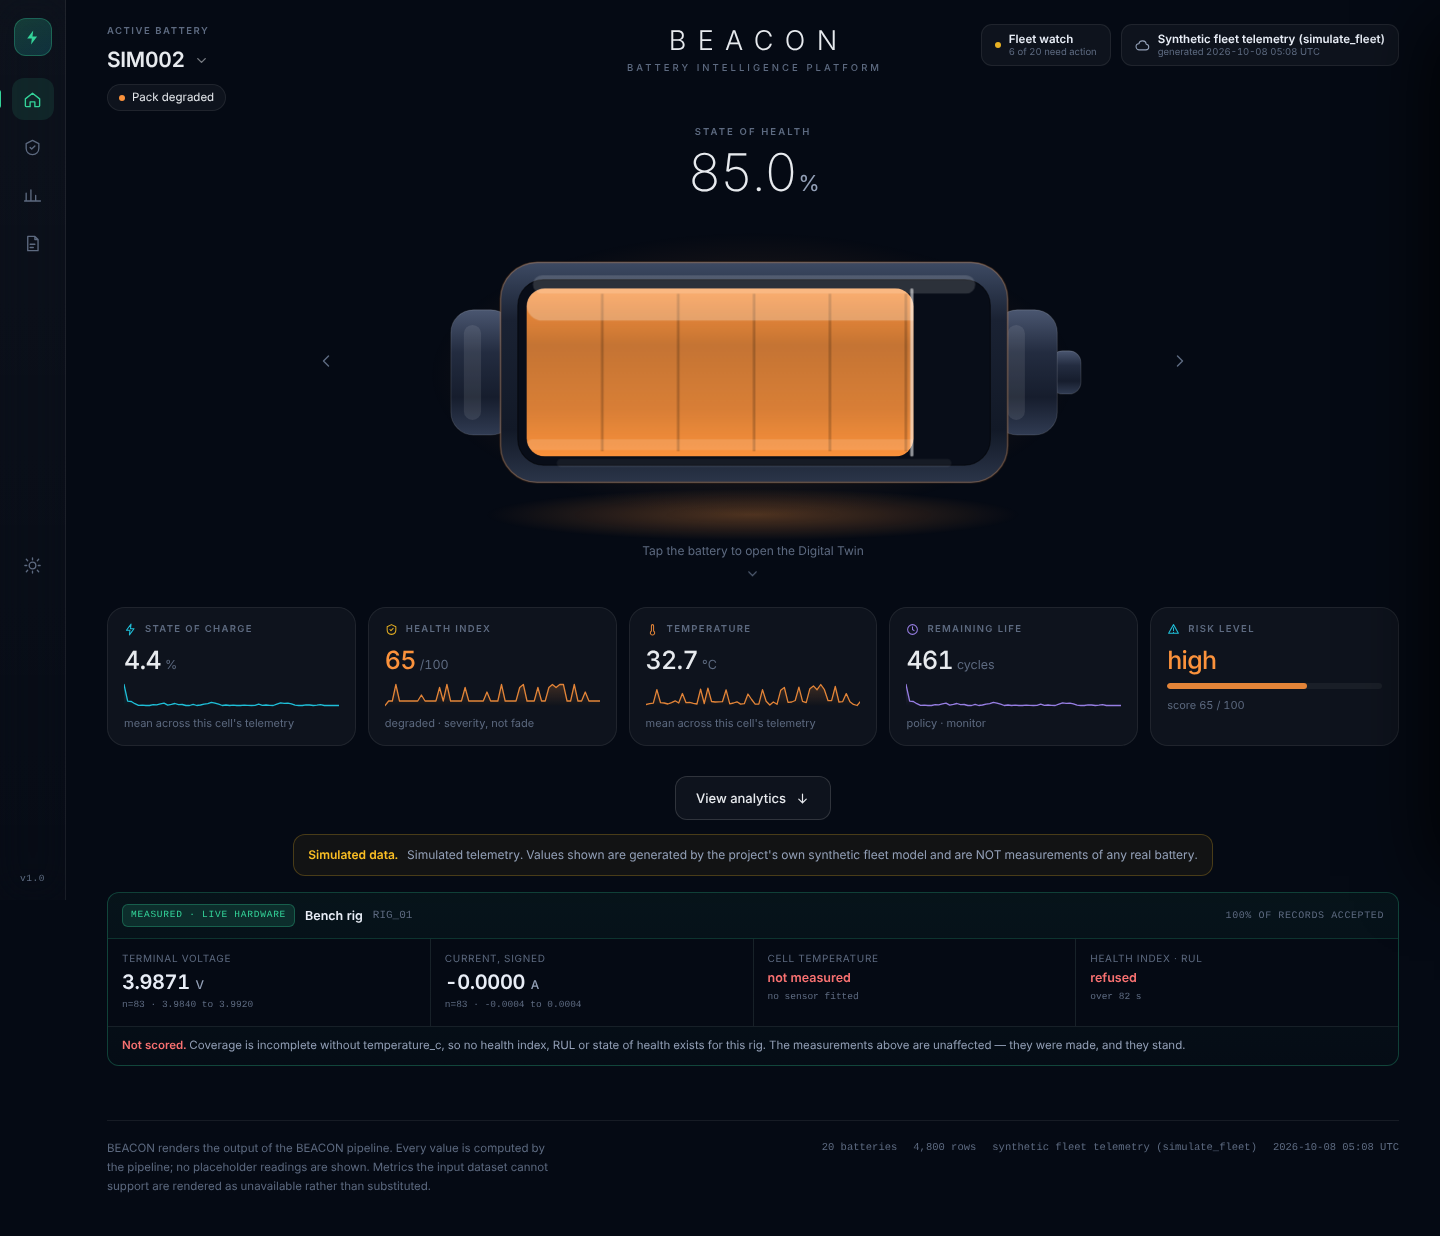
\includegraphics[width=\linewidth,height=0.5\textheight,keepaspectratio]{images/ui_overview.png}
    \caption{Overview screen of the BEACON dashboard on a synthetic fleet. The banner marks the values as simulated, and the panel at the bottom shows the measured bench-rig readings, with the health index and remaining life refused because no temperature channel exists.}
    \label{fig:uioverview}
\end{figure}

\begin{figure}[htbp]
    \centering
    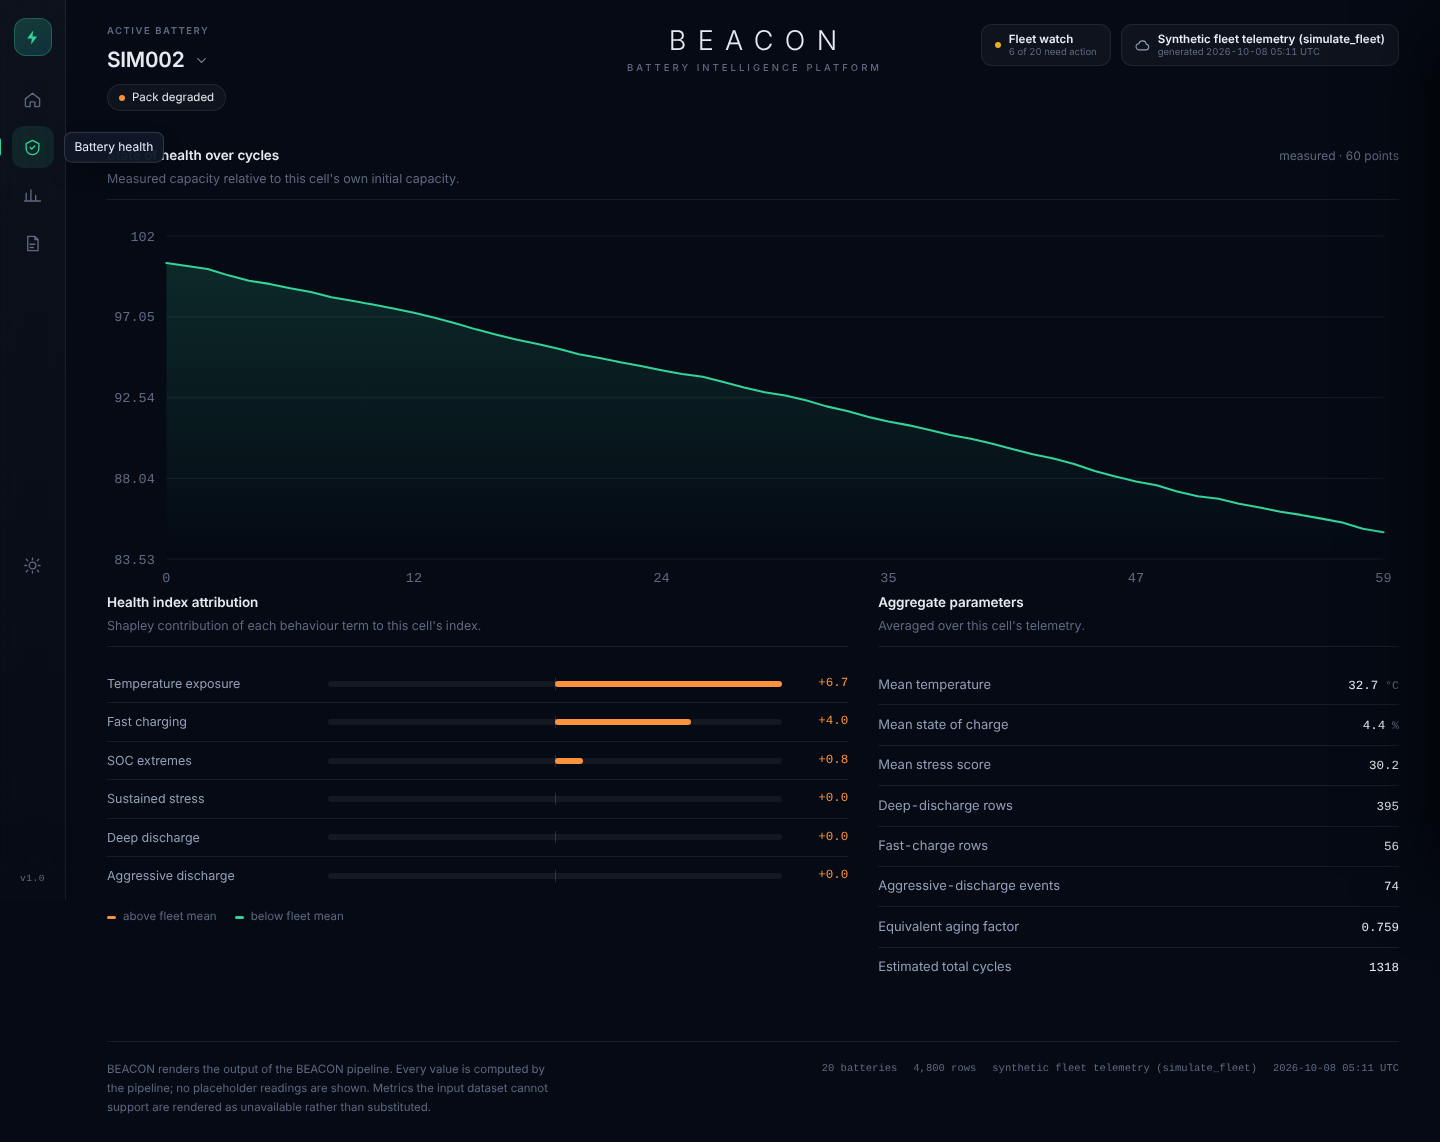
\includegraphics[width=\linewidth,height=0.5\textheight,keepaspectratio]{images/ui_health.png}
    \caption{Battery health screen: state of health over cycles for one battery, the attribution of its health index to behaviour terms, and its aggregate usage parameters (synthetic fleet).}
    \label{fig:uihealth}
\end{figure}

There are two deliberate absences. There is no database: the fleet store is in memory, and adding a database to the compose file would imply a persistence layer that does not exist, so the compose file says so. Persistence is the next substantial piece of work.

\section{DIGITAL TWIN AND FLEET STORE}

The twin is implemented as a domain module with no transport dependency. The API layer is a thin adapter over it, so adding another front end, for example a message broker, means writing a new adapter and leaves the module unchanged. The fleet store holds the latest twin state, the transition history and the telemetry of the most recent run for each battery. It is held in process memory and does not survive a restart, which is stated in the API documentation and shown in the compose file by the absence of a database service.

The twin also carries a field called evidence confidence, which takes one of four values: validated, heuristic, mixed or not applicable. It states whether the causes the Guardian identified for a battery are supported by the calibration work or are hand-chosen thresholds. Temperature exposure is the only cause with a measured, cohort-controlled effect (0.0038~Ah per $^\circ$C), while the current-based causes and the health index itself are marked heuristic. This does not change what the Guardian detects. It changes what the system says about its own certainty, which was previously not visible in the output.

\section{API REFERENCE}

Table~\ref{tab:api} lists the principal routes of the Python service. Further routes cover live CAN capture, serial emulation, live serial capture, latest and live state, thermal and twin views, transfer feasibility and the dataset listing. The interactive documentation generated by FastAPI from the same code is served at \texttt{/docs}, so it cannot drift from the code in the way a hand-written reference can.

\begin{table}[htbp]
	\caption{Principal Routes of the Python Service}
	\centering
	\small
	\renewcommand{\arraystretch}{1.15}
	\setlength{\tabcolsep}{4pt}
	\begin{tabular}{|L{0.4\linewidth}|L{0.4\linewidth}|}
		\hline
		\textbf{Route} & \textbf{Purpose} \\
		\hline
		\texttt{GET /healthz} & Service liveness, with run and battery counts \\
		\hline
		\texttt{POST /pipeline/simulate} & Score a simulated fleet and fold it into the store \\
		\hline
		\texttt{GET /batteries} & Twin state of every battery seen \\
		\hline
		\texttt{GET /batteries/\{id\}} & Twin, Guardian report, risk, history, evidence confidence \\
		\hline
		\texttt{GET /batteries/\{id\}/timeline} & Per-cycle stress, state of charge and temperature \\
		\hline
		\texttt{POST /telemetry/replay} & Replay a recorded CAN log through the pipeline \\
		\hline
		\texttt{POST /telemetry/serial/replay} & Replay a recorded serial capture \\
		\hline
		\texttt{GET /telemetry/coverage} & Report which required signals a DBC file provides \\
		\hline
	\end{tabular}
	\label{tab:api}
\end{table}

A battery that is in the store but absent from the most recent run has a twin state and a history but no timeline, and a request for its timeline returns a not-found response and not a stale series. Every request body is validated by Pydantic. The duration of a live capture is bounded above by 300~s, the number of emulated cycles lies between 1 and 50, the sampling period lies between 0 and 3600~s and the accepted fraction lies between 0 and 1, so no request can start a capture that never returns.

\section{SECURITY CONSIDERATIONS}

The service is a local bench and analysis tool, and its security review asked a narrow question: can a caller who reaches the service make it do something it should not? The review was carried out against the repository and recorded, with the findings and the decision taken on each. Table~\ref{tab:security} summarises them.

\begin{table}[htbp]
	\caption{Security Review of the Service}
	\centering
	\footnotesize
	\renewcommand{\arraystretch}{1.1}
	\setlength{\tabcolsep}{3pt}
	\begin{tabular}{|L{0.3\linewidth}|L{0.5\linewidth}|}
		\hline
		\textbf{Finding} & \textbf{Outcome} \\
		\hline
		Request-supplied file paths on replay and coverage routes & Fixed: path must resolve under an allowed root \\
		\hline
		Cross-origin policy permissive by default & Made configurable; not presented as a security boundary \\
		\hline
		Secrets and language-model integration & Verified absent by search of the repository \\
		\hline
		Request validation & Adequate; bounds on durations and counts \\
		\hline
		Serial parser under adversarial input & Safe: bad lines counted, values rejected, capture refused below a threshold \\
		\hline
		Notebook metadata & Noted; left to the author \\
		\hline
	\end{tabular}
	\label{tab:security}
\end{table}

The one substantive finding was that three routes opened a filesystem path taken from the request body without any containment. A caller could name a private key or a configuration file, and the per-line rejection reasons returned by the serial path could carry fragments of what was read. The difference between a not-found and a parse error also revealed whether a file existed. The fix resolves the path first and requires it to lie under an allowed root, and rejects it with a client error before any existence check, so an out-of-bounds path cannot be used to probe the disk. A list of allowed roots was chosen over a blocklist of path patterns, because blocklists on path strings can be defeated by symbolic links, percent-encoding and short file names, whereas resolving first and then asking where the path ended up is decided after any such trick has been applied. The allowed roots can be replaced through an environment variable, and the variable replaces the defaults and does not extend them, so setting it cannot leave a development convenience in place. Thirteen tests cover the containment.

\subsection{Threats Outside the Scope of the Design}

The service has no authentication, no rate limiting, no transport security and no tenant isolation, and it keeps one global in-memory store. These are consequences of its scope as a local tool and are recorded as such. The correct remedy for a shared deployment is an authenticating reverse proxy in front of the service and not code inside it.

\section{DASHBOARD COMPONENTS}

The dashboard is a React application with one surface, rendered from the pipeline output. Table~\ref{tab:components} lists its views. (The repository also keeps earlier per-panel components that the current surface no longer uses.) The panels that display a measured result carry the provenance of the value, so a reader can tell whether a figure comes from a vehicle, a rig, a dataset or a simulation.

\begin{table}[htbp]
	\caption{Views of the Dashboard}
	\centering
	\small
	\renewcommand{\arraystretch}{1.15}
	\setlength{\tabcolsep}{4pt}
	\begin{tabular}{|L{0.3\linewidth}|L{0.44\linewidth}|}
		\hline
		\textbf{View} & \textbf{Content} \\
		\hline
		Fleet risk distribution & Risk category of every battery \\
		\hline
		Behaviour flag incidence & How often each flagged behaviour occurs \\
		\hline
		Battery health & Stress score over cycles, risk and health-index attribution \\
		\hline
		Aggregate parameters & Usage parameters of the selected battery \\
		\hline
		Guardian explanation & Plain-language report of the causes found \\
		\hline
		Bench rig panel & Measured readings, with refusals shown where a channel is missing \\
		\hline
		Twin sheet & Observed and predicted state; shows not available until the twin is wired in \\
		\hline
		Provenance banner & Source of the displayed values \\
		\hline
	\end{tabular}
	\label{tab:components}
\end{table}

The design mock-up of the dashboard contained placeholder readings, such as a state of health of 92.4\% and a remaining life of 1,245 cycles. A decision record fixes that the interface renders only values that were computed, and shows a refusal or an empty state in place of a placeholder when the pipeline has produced nothing. This is the same stance as in the estimators, applied to the display.

\section{HEALTH REPORT CARD}
\label{sec:impl-card}

The health report script renders the outputs as a plain-language card for one battery, in five parts: how healthy it is, how long it has left, what the usage is doing to it, what to do, and what the report cannot tell. Every figure carries its validation error band, which is taken from a file of measured bands and pinned by a test, and each output is labelled measured, estimate or heuristic. When ground truth exists, the card is followed by a check against the laboratory, which the card itself was not shown. Section~\ref{sec:res-card} reports a worked example.

\section{TESTING, CONTINUOUS INTEGRATION AND REPRODUCIBILITY}
\label{sec:impl-test}

There are 44 test modules, and three kinds of test are not the usual kind.

\begin{itemize}
    \item \textbf{Prose-to-evidence pinning.} A test ties every figure quoted in the documentation to the artifact that produced it, so re-running an experiment and forgetting to update a paragraph fails the build. It caught a stale figure that had already been published.
    \item \textbf{Cross-artifact structural tests.} The firmware's declared field set is compared as a set against the schema, and the documented schema table must equal the rendered one. Substring assertions had already let a defect through: a renamed field left the schema id untouched, so the sketch kept announcing a version it no longer spoke.
    \item \textbf{Known-defect pins.} Some tests assert behaviour that is not desirable, with a comment saying so, for example that the risk score is too coarse to see a sevenfold change in average stress. Changing it would silently re-score every published figure, so it is pinned and a future change has to be deliberate.
\end{itemize}

Continuous integration runs eight jobs: lint and type checking, the test suite on Python 3.10 and 3.12, a job that uninstalls the optional CAN dependency and re-runs the suite, a job that reproduces the headline benchmark end to end, a firmware compile for three targets, the gateway tests, the client build, and the Docker build. The job without the optional dependency exists because ``it is optional'' is otherwise an untested claim. The Python-version matrix exists because testing only the newest version lets a declared floor rot silently.

\subsection{Test Modules by Subsystem}

Table~\ref{tab:tests} lists some of the test modules and the behaviour each one pins. Each subsystem has tests at its own boundary, so a fault is caught where it is introduced and not where it is first noticed.

\begin{table}[htbp]
	\caption{Selected Test Modules and Verified Behaviour}
	\centering
	\footnotesize
	\renewcommand{\arraystretch}{1.1}
	\setlength{\tabcolsep}{3pt}
	\begin{tabular}{|L{0.42\linewidth}|L{0.42\linewidth}|}
		\hline
		\textbf{Module} & \textbf{Behaviour checked} \\
		\hline
		\texttt{test\_api} & Route behaviour, repeated identical seeded run produces no new twin transitions \\
		\hline
		\texttt{test\_api\_path\_containment} & Absolute sensitive paths, parent-directory traversal and empty paths are rejected before any existence check; the environment-variable override is covered \\
		\hline
		\texttt{test\_can\_dbc} & Decoded values match the published worked example; missing voltage and temperature reported by the validator \\
		\hline
		\texttt{test\_can\_vehicle\_registry} & Vehicle identified from observed identifiers; ambiguous input refused \\
		\hline
		\texttt{test\_digital\_twin} & State derivation and transition recording \\
		\hline
		\texttt{test\_serial\_telemetry} & Framing, checksum, rejected values, capture-level refusal \\
		\hline
		\texttt{test\_hardware\_readiness} & Truncated lines, corrupted checksums, non-finite and out-of-range fields \\
		\hline
		Gateway tests (\texttt{gateway}, \texttt{telemetry}) & Each route forwards to the Python service and returns its result unchanged \\
		\hline
	\end{tabular}
	\label{tab:tests}
\end{table}

\section{CONTAINERISATION AND DEPLOYMENT}
\label{sec:impl-deploy}

The Docker image is multi-stage on a slim Python 3.12 base, with the compiler confined to the build stage, a non-root user, and a health check that polls service liveness. Docker Compose brings up the API, the gateway and the client, with the gateway held until the API reports healthy, and a separate study service writes the result CSVs back to the host. The system runs on a fresh clone with no hardware, no database, no API keys and no dataset download:

\begin{verbatim}
python main.py                     # end-to-end run
python scripts/run_serial_demo.py  # emulated rig
python -m pytest tests/ -q         # the test suite
docker compose up                  # API, gateway, client
\end{verbatim}

\section{OPERATIONAL WORKFLOW}

A typical session with the system follows the same path whatever the source. An operator starts the three services, or runs the single command that produces the end-to-end result, and selects a source: a simulated fleet, a recorded CAN log with its DBC file, a serial capture, or a live capture from the rig. The service converts the source to the unified frame, applies the schema and capture-level checks, and scores the result. The dashboard then shows the fleet table first, with each battery's health, risk and remaining life, and each value labelled with its source. Selecting a battery opens its detail, where the health over cycles, the attribution of the health index and the twin history are shown. If a capture was refused, the dashboard shows the refusal and its cause in the place where the number would have been.

The same path serves a bench session. With the rig connected, the operator records a capture to a file and replays it through the serial route, which gives the same result as scoring it live and leaves a file that can be re-scored after any change to the code. Replay from a recorded file is also how the results of this report were reproduced, since a file scored twice gives the same output, and a live cell does not.

\section{CHAPTER SUMMARY}

This chapter described the realisation of the design: a shared scoring path fed by three transports through a narrow seam, a self-synchronising wire protocol with refusal gates at both record and capture level, a physical rig brought up in two stages, a three-service stack served from containers, and a test and CI strategy aimed at keeping the documentation and the code honest. What this implementation \emph{achieved} is reported in the next chapter.
